%!TEX root =../../../course-notes.tex
% ^ leave for LaTeXTools build functionality

\begin{applicationActivities}



\begin{definition}
  A subset of a vector space is called a \term{subspace} if it is
  a vector space on its own.

  \vspace{1em}

  For example, the span of these two vectors forms a planar subspace
  inside of the larger vector space \(\IR^3\).

  \begin{center}
  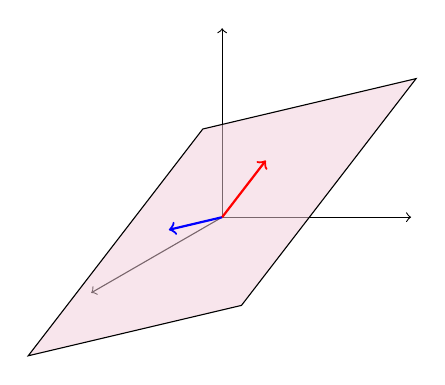
\begin{tikzpicture}[x={(210:0.8cm)}, y={(0:1cm)}, z={(90:1cm)},scale=0.4]
    \draw[->] (0,0,0) -- (6,0,0);
    \draw[->] (0,0,0) -- (0,6,0);
    \draw[->] (0,0,0) -- (0,0,6);
    \draw[fill=purple!20,fill opacity=0.5]
      (-2,-2,2) -- (6,-2,-2) -- (2,2,-2) -- (-6,2,2) -- (-2,-2,2);
    \draw[thick,blue,->] (0,0,0) -- (1,-1,0);
    \draw[thick,red,->] (0,0,0) -- (-2,0,1);
  \end{tikzpicture}
  \end{center}
\end{definition}



\begin{fact}
  Any sub\textbf{set} \(S\) of a vector space \(V\) that contains
  the additive identity \(\vec 0\) satisfies the eight
  vector space properties automatically, since it is a collection of known
  vectors.

  \vspace{1em}

  However, to verify that it's a sub\textbf{space}, we need to check that
  addition and multiplication still make sense using only vectors from \(S\).
  So we need to check two things:

  \begin{itemize}
  \item The set is \textbf{closed under addition}: for any \(\vec{x},\vec{y} \in S\), the sum \(\vec{x}+\vec{y}\) is also in \(S\).
  \item The set is \textbf{closed under scalar multiplication}: for any \(\vec{x} \in S\) and scalar \(c \in \IR\), the product \(c\vec{x}\) is also in \(S\).
\end{itemize}
\end{fact}

\begin{activity}{15}
Let \(S=\setBuilder{\begin{bmatrix} x \\ y \\ z \end{bmatrix}}{ x+2y+z=0}\).

\begin{subactivity}
  Let \(\vec{v}=\begin{bmatrix} x \\ y \\ z \end{bmatrix}\) and
  \(\vec{w} = \begin{bmatrix} a \\ b \\ c \end{bmatrix} \) be vectors in \(S\),
  so \(x+2y+z=0\) and \(a+2b+c=0\). Show that
  \(\vec v+\vec w = \begin{bmatrix} x+a \\ y+b \\ z+c \end{bmatrix}\)
  also belongs to \(S\) by verifying that \((x+a)+2(y+b)+(z+c)=0\).
\end{subactivity}
\begin{subactivity}
  Let \(\vec{v}=\begin{bmatrix} x \\ y \\ z \end{bmatrix}\in S\), so
  \(x+2y+z=0\). Show that \(c\vec v=\begin{bmatrix}cx\\cy\\cz\end{bmatrix}\) 
  also belongs to \(S\) for any \(c\in\IR\) by verifying
  an appropriate equation.
\end{subactivity}
\begin{subactivity}
  Is \(S\) is a subspace of \(\IR^3\)?
\end{subactivity}
\end{activity}

\begin{activity}{10}
Let \(S=\setBuilder{\begin{bmatrix} x \\ y \\ z \end{bmatrix}}{ x+2y+z=4}\).
Choose a vector
\(\vec v=\begin{bmatrix} \unknown\\\unknown\\\unknown \end{bmatrix}\) in \(S\)
and a real number \(c=\unknown\), and show that \(c\vec v\) isn't in \(S\).
Is \(S\) a subspace of \(\IR^3\)?
\end{activity}

\begin{remark}
Since \(0\) is a scalar and \(0\vec{v}=\vec{z}\) for any vector \(\vec{v}\), a
nonempty set that is closed under scalar multiplication must contain the zero vector
\(\vec{z}\) for that vector space.

\vspace{1em}

Put another way, you can check any of the following to show that a
nonempty subset \(W\) isn't a subspace:

\begin{itemize}
  \item Show that \(\vec 0\not\in W\). 
  \item Find \(\vec u,\vec v\in W\) such that \(\vec u+\vec v\not\in W\).
  \item Find \(c\in\IR,\vec v\in W\) such that \(c\vec v\not\in W\).
\end{itemize}

If you cannot do any of these, then \(W\) can be proven to be a subspace
by doing the following:
\begin{itemize}
  \item Prove that \(\vec u+\vec v\in W\) whenever \(\vec u,\vec v\in W\).
  \item Prove that \(c\vec v\in W\) whenever \(c\in\IR,\vec v\in W\).
\end{itemize}
\end{remark}

\begin{activity}{20}
  Consider these subsets of \(\IR^4\):
  \[
    R=
    \setBuilder{ \begin{bmatrix}x\\y\\z\end{bmatrix}}{y=z+1}
    \hspace{2em}
    S=
    \setBuilder{ \begin{bmatrix}x\\y\\z\end{bmatrix}}{y=|z|}
    \hspace{2em}
    T=
    \setBuilder{ \begin{bmatrix}x\\y\\z\end{bmatrix}}{z=xy}
  \]
  \begin{subactivity}
  Show \(R\) isn't a subspace by showing that \(\vec 0\not\in R\).
  \end{subactivity}
  \begin{subactivity}
  Show \(S\) isn't a subspace by finding two vectors \(\vec u,\vec v\in S\)
  such that \(\vec u+\vec v\not\in S\).
  \end{subactivity}
  \begin{subactivity}
  Show \(T\) isn't a subspace by finding a vector \(\vec v\in T\)
  such that \(2\vec v\not\in T\).
  \end{subactivity}
\end{activity}



\begin{activity}{5}
Let \(W\) be a subspace of a vector space \(V\).  How are \(\vspan W\) and \(W\) related?
\begin{enumerate}[(a)]
\item \(\vspan W\) is bigger than \(W\)
\item \(\vspan W\) is the same as \(W\)
\item \(\vspan W\) is smaller than \(W\)
\end{enumerate}
\end{activity}

\begin{fact}
  If \(S\) is any subset of a vector space \(V\), then
  since \(\vspan S\) collects all possible linear combinations,
  \(\vspan S\) is automatically a subspace of \(V\).

  \vspace{1em}

  In fact, \(\vspan S\) is always the smallest
  subspace of \(V\) that contains all the vectors in \(S\).
\end{fact}

\end{applicationActivities}
